\chapter{Исскуство}

\section{Дадаизм: история, основы и суть}

\textit{Источник: \url{https://4brain.ru/blog/dadaizm-istoriya-osnovy-i-sut/}}

Группа молодых людей дружно хохотала, сидя за столиком маленького кафе и обсуждая политику, африканскую музыку, скульптуру и \ex{ударные}{drums, percussion}. Все они сбежали от войны в эту нейтральную страну, чтобы жить, \ex{творить}{to create} и радоваться. И это не Дубай наших дней, а Цюрих вековой давности. В Первую мировую войну в его переулках родилось течение дадаистов, которые открыли новую главу в культуре Запада. Они научили людей думать и чувствовать по-другому.

\textbf{История дадаизма.}
Дадаизм \ed{многолик}{многоликий}{multifaceted, many-sided}. В этом стиле творили десятки, сотни людей в самых разных странах Европы и Америки. Каждый из них \ex{внес свою лепту}{made his contribution} в течение, но это же и стало его проклятием: т.к. у движения не было лидера, после завершения Первой мировой войны дадаисты разъехались по всему миру, от Японии до США, и стали творчески \ex{переосмысливать идеи}{to rethink ideas}, зародившиеся в Цюрихе.

У \ed{истоков}{исток}{место, где начинается водный источник (река, ручей); начало, первоисточник чего-н. («истоки первобытной культуры»)} дадаизма стоял немецкий поэт Хуго Балль. Изначально он поддерживал военню риторику и даже пытался вступить в армию добровольцем. Однако, когда Германия вторглась в Бельгию, Балль перестал поддерживать правящий режим, был назван родной страной предателем, поэтому был вынужден бежать туда, где говорили на его родном немецком языке: в швейцарский Цюрих. С собой Балль прихватил возлюбленную Эмму Хеннингс, которая также была поэтессой, и твердое убеждение, что война --- это зло.

\ex{Осев}{From the verb осесть: to settle} на берегах Цюрихского озера, влюбленные познакомились с владельцем винного погребка Meierei на улице Шпигельгассе. Он был очарован молодой парой, их \ed{задором}{задор}{enthusiasm} и творческой энергией. Предприниматель прикинул, что если сдаст им один из пустующих залов (совсем маленький, площадью около десяти квадратных метров), то сможет увеличить доходы с продажи пива многочисленным молодым собутыльникам Хуго и Эммы.

Расчет оправдался: владелец-голландец получил свои барыши, а влюбленные – место, которое они превратили в легендарное «Кабаре Вольтер». Сегодня мы бы назвали это место баром или кафе. Однако название было звучным и всем понравилось. Имя философа-просветителя 18 века влюбленные выбрали из-за написанной им повести «Кандид», в которой Вольтер высмеивал религиозные и философские догмы своего времени.

Хуго и Эмму такой подход восхищал и вдохновлял. Они не остановились на религии и философии и за те долгие годы, что по миру грохотала Первая мировая война, переосмыслили догмы Старого Света, дав пищу искусству Нового Света (Америки) и послевоенной Европы.

Первое представление в «Кабаре Вольтер» состоялось 5 февраля 1916 года: молодежь организовала варьете с песнями на французском и немецком языке, русской и африканской музыкой, а также небольшую выставку.

Представление имело огромный успех. Круг общения Хуго и Эммы ширился, в него вливались все новые и новые эмигранты из европейских стран. Местных было очень мало. «Швейцарская молодежь слишком осторожна для кабаре», – таково было мнение Хуго.

Хотя в мире бушевала Первая мировая война, эмигранты не голодали, иногда они ели стейки, запивали их хорошим испанским вином и праздновали подобающим образом. Молодые люди зарабатывали пером, игрой на пианино в пабах, рисовали для богатых заказчиков и выполняли другие частные заказы творческого характера.

Как и предсказывал хозяин Meierei, представления «Кабаре Вольтер» пользовались популярностью у населявших в тот момент Цюрих молодых людей, а потому приносили хорошие деньги.

14 июля 1916 года Балль выпустил основополагающий «Манифест Дада». Именно он определил вектор направления дадаизма.

Откуда взялось его название, до конца непонятно. По одной версии, это славянское двойное утверждение (русское «да-да»). По другой, это детская игрушечная лошадка на французском языке. Существует с десяток других версий. Как истинные творцы, дадаисты выступали за плюрализм мнений.

\textbf{Лица дадаизма.} Балль оказался не только талантливым организатором, но и поэтом-новатором. В Европе его считают одним из создателей так называемой «фонетической поэзии». Он писал строки наподобие:

«Gadji beri bimba glandridi laula lonni cadori

gadjama gramma berida bimbala glandri galassassa laulitalomini

gadji beri bin blassa glassala laula lonni cadorsu sassala bim».

Эти слова никак не переводятся. Балль изобрел каждое из них. Это «стихи без слов». В строках нет смысла, но в этом и вся прелесть. Носителю славянских языков эти строки покажутся белибердой, а европейцу – чем-то прекрасным. Поэма будет иметь огромный успех в западной культуре и в 21 веке, когда дадаистам посвятят очередной Ноттинг-Хиллский карнавал.

«Сколько слов и словосочетаний можно вытащить из этого калейдоскопа? Это зависит от того, на какие языки и диалекты мы можем ссылаться (и является ли «Нонсенс» одним из них). Как на карнавале, где на каждом углу соперничают многочисленные оркестры и звуковые системы, зевакам приходится постоянно настраивать свои внутренние наушники.

Вы можете уловить в этих строках немного латыни, греческого, итальянского, румынского, шведского (возможно), турецкого, немецкого (конечно) и английского, – и подозревать, что вы все еще прочесываете только верхушку айсберга», – так охарактеризовала эти строки Балля его современная коллега из Великобритании Кароль Руменс [The Guardian, 2009].

Ближайшим соратником Хуго по кружку дадаистов стал выросший в Румынии артист Тристан Тцара. Он родился в еврейской семье под именем Самуэль Розеншток, а евреям в Королевстве Румыния не полагались полные гражданские права. Когда началась война, Самуэль порвал с родиной и стал творить на чужбине на французском языке. Именно Тцара выпустит вторую часть «Манифеста Дада» и продолжит дело Хуго, когда тот женится на Эмме и отойдет от дел «Кабаре Вольтер».

Значительный вклад в стиль дадаизма внесли скульпторы Марсель Янко и Жан Арп.

Особняком стоял французский художник Марсель Дюшан, который вместе с Пабло Пикассо и Анри Матиссом определит революционные разработки в пластическом искусстве 20 века. Пририсовать «Моне Лизе» усики и бородку? Очень в стиле Дюшана. Сегодня это творение выставлено на почетном месте в парижском Центре Помпиду (Рис \ref{fig:mona-lisa})
\begin{figure}
    \centering
    \includegraphics[width=0.7\textwidth]{img/pompidou.jpg}
    \caption{Mona Lisa}\label{fig:mona-lisa}
\end{figure}


Поддержку дадаистам выражали:
\begin{enumerate}
    \item Цюрихский врач для бедных, социалист Фриц Брупбахер.
    \item Директор цюрихской школы имени Иоганна Генриха Песталоцци, галерист Хан Корай. Именно он предоставил дадаистам свою галерею в отличном месте, в доме Шпрюнгли, для выставок, мероприятий и крупных фестивалей «Дада».
    \item Анархист Юлиус Хойбергер разрешит дадаистам пользоваться своей типографией. Т.к. многие работы дадаистов были сложными по графике, хороший результат требовал сотрудничества издателя и творца.
    \item Местная пресса. Хотя во многих странах молодых дадаистов представляют как аморальных пьяниц, швейцарские журналисты того времени в целом относились к движению «Дада» с пониманием и уважением. «Редакция одного из ведущих швейцарских СМИ, которое с успехом переживет 20 век, Neue Zürcher Zeitung, и вовсе выражала дадаистам свою благосклонность», – подчеркивают их коллеги из швейцарского журнала Schweizer Monat, который выходит в Цюрихе с 1921 года [B. Ruetz, 2003].
\end{enumerate}

С «Кабаре Вольтер» сотрудничали: (i) Василий Кандинский, (ii) Амедео Модильяни, (iii) Пабло Пикассо, (iv) Гийом Аполлинер, (v) Филиппо Томмазо Маринетти.

Само «кабаре» на улице Шпигельгассе просуществует недолго, всего полгода: открывшись зимой 1916 году, уже осенью того года его не станет. Дадаистов развелось так много, что им стало банально тесно на десяти квадратных метрах. Последний перфоманс «Кабаре Вольтер» пройдет летом 1916 года. В 1917 году была открыта Галерея Дада.

\textbf{Протест искусства или искусство протеста?}
Дадаизм – сын Первой мировой войны. Дадаизм в искусстве возник из разочарования миром, который допустил войну.

Многие дадаисты считали, что «разум» и «логика» буржуазного капиталистического общества привели людей к войне. Они выражали свое неприятие этой идеологии в художественном выражении, которое, казалось, отвергало логику и принимало хаос и иррациональность. Например, немецкий карикатурист Джордж Гросс позже вспоминал, что его дадаистские творения были задуманы как протест «против этого мира взаимного уничтожения».

Для дадаизма характерно противостояние позитивизму, научному мышлению, основанному на понятии разума, а также литературным и художественным традициям, чистоте отвлеченных понятий.

Поэтому дадаизм исходил из необходимости порвать с устоявшимися тенденциями и способствовать анархии в художественном мире, даже навязывая идеологию и новый образ жизни, в которых отвергались традиционное и условное.

Немецкий художник Ханс Рихтер и вовсе утверждал, что дадаизм не был искусством: он был «антиискусством».

Дадаизм представлял собой противоположность всему, что символизировало искусство. Там, где искусство было связано с традиционной эстетикой, дадаисты игнорировали эстетику. Если искусство должно было воздействовать на чувства, то дадаизм должен был оскорбить.

Кроме того, стиль «Дада» попытался отразить человеческое восприятие и хаотичную природу общества.

Как выразился Балль: «Для нас искусство не самоцель… но это возможность для истинного восприятия и критики времени, в котором мы живем» [Национальная галерея искусства в Вашингтоне, 2006].

С точки зрения дадаистов, массовое искусство и культура их времени представляли собой фетишизацию, когда объекты потребления (включая организованные системы мысли, такие как философия и мораль) выбираются так же, как торт или сорт вишни, чтобы заполнить пустоту.

\textbf{Характеристики и основы дадаизма.}
Дадаизм и искусство дадаизма не определяли единого стиля, поскольку основывались именно на критике традиционного чувства искусства, школы или стиля. Тем не менее, направление дадаизма объединено рядом общих принципов, придававших ему характерный тон как в литературном, так и в пластическом плане:
\begin{enumerate}
    \item Междисциплинарный характер. Практически никто из дадаистов не творил только в одном жанре. Тот же Балль, помимо поэзии, был успешным журналистом, эссеистом, драматургом. Именно дадаисты придумали объединить фотографию и скульптуру.
    \item Отвращение концепции красоты. Для дадаистов традиционная концепция искусства потеряла смысл перед лицом реальности насилия, развязанного в Европе. Молодые люди считали, что искать красоту и ублажать чувства недопустимо перед лицом ужасов войны.
    \item Антихудожественный и антилитературный смысл. Т.к. дадаизм позиционировал себя как «антиискусство», для его понимания больше важны не формы, а концепция, способ воздействия на реальность.
    \item Оценка художественного жеста выше художественного объекта. Дадаисты верили, что художник перестанет быть тем, кто рисует или ваяет, тем, кто творит красоту, и станет тем, кто выбирает предмет без эстетических претензий и придает ему смысл уже в самом факте своего выбора. Таким образом устанавливается эпоха, в которой жест художника будет действительно считаться «художественным».
    \item Ироничный, провокационный и дерзкий юмор. Дадаизм предложил свирепое издевательство над искусством – не только традиционным искусством, но и авангардным искусством, таким как кубизм и футуризм (последний прославлял войну).
    \item Острая критика западного общества. Предложение «Дада» построено как отказ от буржуазных ценностей начала века: слепой и бездумной веры в научно-техническое развитие как смысл истории, радикального национализма, культа капитала и использования искусства как транквилизатора совести.
    \item Заявление об иррациональности как отказ от позитивизма. Поняв, что человеческий разум принес с собой не лучшую жизнь, а массовые разрушения, дадаисты стали настаивать, что искусство и литература больше не должны оправдываться именем разума. Таким образом, они возвели в приоритет иррациональность и абсурд. Этот способ работы сделал возможным беспрецедентное творческое развитие, хотя и не был свободен от споров и неприятий.
    \item Создание новых художественных техник. Дадаисты популяризировали каллиграфию Аполлинера и созданный кубистами коллаж, изобрели фотомонтаж и реди-мейд (создание предмета искусства из повседневного объекта, например, писсуара).
    \item Инновационное использование слова. Привязанный к ценностям движения, дадаизм предпочитал использование слов по очереди, не будучи связанным очевидным значением или логическим дискурсивным смыслом. В качестве исходного материала они также брали сами буквы и звуки, что позволяло избежать ассоциации с рациональным смыслом. Важную роль в этом сыграла случайность.
\end{enumerate}
Дадаизм – это не столько художественный жанр, сколько образ жизни. Молодые творцы ценили спонтанность, импровизацию, отказ от традиций. Причем, везде. В том числе в музеях. Именно они первыми стали использовать мусор в искусстве.

Дадаисты отказывались творить и думать по шаблону и учили этому других. Их эксперименты так вдохновят Запад, что «разрыв шаблона» станет устойчивым выражением у западных людей и даст начало популярной ныне теории когнитивного диссонанса. Если вы думаете, что это одно и то же, но сомневаетесь и хотите знать точно, как достичь консонанса, записывайтесь на нашу онлайн-программу «Когнитивистика».

Дадаисты обожали:
провокации,
эпатаж,
демонстрации,
перфомансы,
скандалы,
фантастику,
экспрессию,
несовершенство,
естественность.

Поэтому в своей отрицательной строгости дадаизм выступал против модернизма и различных авангардных течений: экспрессионизма, кубизма, футуризма и абстракционизма, обвиняя их, в конечном счете, в том, что они являются заменителями того, что было уничтожено или вот-вот будет уничтожено.

Главный вклад дадаизма в современное искусство заключается в том, что дадаисты поставили вопрос о том, что такое искусство или что такое поэзия, привели людей к пониманию того, что все есть условность, которую можно подвергнуть сомнению, и, следовательно, не существует фиксированных и вечных правил, исторически узаконивающих художественное. Многое из того, что является провокационным в современном искусстве (например, смешение жанров и материалов, типичное для коллажа), происходит из дадаизма.

Хотя дадаисты использовали революционные методы, их идеи были основаны на глубокой вере, восходящей к романтической традиции, в присущую человечеству доброту, пока та не была испорчена обществом.

\textbf{География послевоенного дадаизма.}
Возникнув в Швейцарии в 1916 году в «Кабаре Вольтер», где был обнародован первый «Манифест Дада», дадаизм распространился по всей планете. После того, как Первая мировая война закончилась, цюрихские дадаисты разъехались по миру. Дадаизм в искусстве стал исключительно городским феноменом.


\textit{Дадаизм в Германии.}
5 июня 1920 года в Берлине прошла Международная ярмарка Дада. Центральной фигурой выставки стала свисающая с потолка фигура немецкого офицера с головой свиньи (Рис. \ref{fig:damaism-germany}).

\begin{figure}[h]
    \centering
    \includegraphics[width=0.7\textwidth]{img/dadaism-germany.jpg}
    \caption{Дадаизм в Германии}\label{fig:damaism-germany}
\end{figure}

Помимо перфомансов и прочего творчества, переехавших в послевоенную Германию дадаистов живо интересовала политика. Идеологически позиции художников-дадаистов были коммунистическими, а в некоторых случаях и анархистскими. Дадаисты занимали устойчивый левый сектор.

Дадаизм окончательно пустит корни в Германии, когда местный поэт Рихард Хюльзенбек выпустит немецкий манифест ДаДа и начнет издавать «Альманах Дада». До своей смерти в 1974 году Хюльзенбек будет повторять, что «ДаДа еще жив».

Именно немецкие дадаисты придумают использовать технику фотомонтажа и коллажа, чтобы запечатлеть окружающую их действительность, используя визуальный материал, взятый из СМИ.

\textit{Дадаизм в США.}
Европейские беженцы Дюшан, Пикабиа, Мина Лой и Жан Кротти вместе с американскими артистами Ман Рэем, Беатрис Вуд, Мортоном Шамбергом, Эльзой фон Фрейтаг-Лорингховен, Флориной Стеттхаймер дадут жизнь нью-йоркскому дадаизму.

Американские дадаисты примкнут к авангардным течениям, которые назревали в Гарлеме, Гринвич-Виллидж и Чайнатауне с начала века.

\textit{Дадаизм во Франции.}
Париж стал новым центром дадаизма в 1920 году.

Вдохновленные Тристаном Тцарой, французские дадаисты издавали манифесты, организовали демонстрации, ставили спектакли и выпускали журналы в стиле дадаизма.

В 1921 году дадаисты представят парижской публике свои работы в рамках Салона Независимых. Пьеса «Газовое сердце» Тцары вызовет бурю насмешек, а затем и целый театральный бунт, который станет началом конца французского движения дадаизм. Сюрреализм – это его детище, которое вырастет на осколках парижского дадаизма.

Ураган дадаизма пронесется по Италии, Японии, Нидерландам, Югославии, Грузии, но Россию не затронет. В молодом советском государстве появится множество сочувствующих дадаизму лиц, однако официально советских творцов к направлению дадаизма не причисляют.

\textit{Космополитизм.}
Как и Сократ с Диогеном, дадаисты много размышляли над свободой отдельного человека и тем, что интересы личности и человечества в целом выше интересов отдельной страны. Европейские дадаисты были искренне уверены, что Западу пора кончать считать себя центром Вселенной, особенно в разгар бушующей войны.

Дадаисты много общались с этнографами, археологами, историками, фольклористами. Музыка и песни дадаистов заимствовали ритмы и костюмы из Африки и Новой Зеландии, которую до прибытия европейцев населял народ маори.

Пытаясь отрицать, а в идеале, низвергнуть западную цивилизацию, дадаисты призывали вернуться к исцеляющим первобытным состояниям, не особенно волнуясь над степенью идеализации этих самых состояний.

Именно здесь оказалась зарыта «культурная бомба». В 21 веке во многих странах «примитивистские» выступления дадаистов считаются оскорбительными. Как и многие современные художники, принявшие «примитивизм», дадаисты присваивали незападные культурные артефакты, не понимая и не признавая их первоначальных ценностей и целей. Они предполагали, что африканские культуры и народы нерациональны, и стремились обобщить все африканские и океанические культуры в единое однородное целое [Khan Academy, Ch. Cramer, K. Grant, 2023].

И хотя дадаисты не стали мировыми знаменитостями, как импрессионисты или философы Древней Греции, они вошли в историю благодаря тому дерзкому вызову, что бросили цивилизованному миру. Их идеи пережили их самих, повлияв на мышление людей в самых разных странах, не только в Европе. Дадаизм 20 века – это не столько про искусство, сколько про человека и его возможности. Именно поэтому дадаизмом так вдохновлялись такие гении 20 века, как Дэвид Боуи и Фрэнк Заппа, пропагандировавший самообразование.

Если вы тоже, как дадаисты, уже подошли к той мысли, что не все в этой жизни обусловлено разумом и логикой, и готовы идти по этой опасной дороге правды до конца, какой бы трудной и непредсказуемой она ни была, нам лишь остается пожелать вам стойкости и храбрости на этом пути.


\newpage
\section{Художники}
\subsection{Виктор Михайлович Васнецов}
% https://muzei-mira.com/biografia_hudojnikov/765-viktor-mihaylovich-vasnecov-biografiya.html
В\'{и}ктор Мих\'{а}йлович Васнец\'{о}в родился в 1848 году 15 мая в селе со смешным названием Лопьял. Отец Васнецова был священником, также как и его дед и прадед. В 1850 году Михаил Васильевич увёз семью в село Рябово. Это было связано с его службой. У Виктора Васнецова было 5 братьев, один из которых также стал знаменитым художников, звали его Аполлинарий.

Талант Васнецова проявился с детства, но крайне неудачное \explainDetail{денежное}{д\'{е}нежный/-ая/-ое}{monetary} положение в семье не оставило вариантов, как отдать Виктора в Вятское духовное училище в 1858 году. Уже в 14-летнем возрасте Виктор Васнецов учился в Вятской духовной семинарии. Детей священников туда брали бесплатно.

Так и не окончив семинарию, в 1867 году Васнецов отправился в Петербург поступать в Академию художеств. Денег у него было совсем мало, и Виктор выставил на «аукцион» 2 свои картины -- «Молочница» и «Жница». До \explainDetail{отъезда}{отъезд}{departure} он так и не получил за них денег. 60 рублей за эти две картины он получил спустя несколько месяцев уже в Петербурге. \explainDetail{Прибыв}{прибывать/прибыть}{arrive} в столицу, у молодого художника было всего 10 рублей.

Васнецов отлично справился с экзаменом по рисованию и сразу \explain{был зачислен}{was enrolled (зачисл\'{я}ть/зач\'{и}слить: to enrol, to enlist)} в Академию. Около года он занимался в Рисовальной школе, где и познакомился со своим учителем -- И. Крамским.

К занятиям в Академии художеств Васнецов приступил в 1868 году. В это время он \explain{сдружился с}{made friends with} Репиным, и даже одно время они жили на одной квартире.

Хоть Васнецову и нравилось в Академии, но он её не закончил, уехав в Париж в 1876 году, где прожил больше года. В это время там же находился и Репин в \explainDetail{командировке}{командировка}{business trip}. Они также поддерживали дружеские отношения.

После возвращения в Москву Васнецова сразу приняли в Товарищество передвижных художественных выставок. К этому времени стиль рисования художника значительно меняется, да и не только стиль, сам Васнецов перебирается жить в Москву, где сближается с Третьяковым и Мамонтовым. Именно в Москве Васнецов \explainDetail{раскрылся}{раскрыв\'{а}ться/раскр\'{ы}ться}{to open, uncover oneself, to come out}. Ему нравилось находиться в этом городе, он чувствовал себя легко и \explainDetail{выполнял}{выполн\'{я}ть/в\'{ы}полнить}{to perform, execute, carry out} различные творческие работы.

Более 10 лет Васнецов \explainDetail{оформлял}{оформл\'{я}ть/оф\'{о}рмить}{put into shape, form} Владимирский соб\'{о}р в Киеве. В этом ему помогал М. Нестеров. Именно после окончания этой работы, Васнецова можно по праву назвать великим русским иконописцем.

1899 год стал \explainDetail{пиком}{пик}{peak} популярности художника. На своей выставке Васнецов представил публике «Трёх богатырей».

После революции Васнецов стал жить уже не в России, а в СССР, что его серьёзно \explainDetail{угнетало}{угнетать}{opress, depress, despirit}. Люди \explainDetail{уничтожали}{уничтож\'{а}ть/уничт\'{о}жить}{to destroy, obliterate; уничтож\'{е}ние: destruction} его картины, \explainDetail{относились}{относ\'{и}ться + \textit{дат.}}{to treat} неуважительно к художнику. Но до конца своей жизни Виктор Михайлович был в\'{е}рен своему делу -- он рисовал. \explainDetail{\'{У}мер}{умирать/умереть}{умир\'{а}ю, умир\'{а}ешь, умир\'{а}ют; умр\'{у}, умрёшь, умр\'{у}т: to die} он 23 июля 1926 года в Москве, так и не закончив портрет своего друга и ученик\'{а} М. Нестерова.



\subsection{Лики России Виктора Васнецова}

17 января в Центральной районной библиотеке им. А. П. Чехова прошла интерактивная лекция «\explainDetail{Лики}{лик}{character (like in a book)} России Виктора Васнецова»

Виктор Васнецов был известным мастером бытовой и исторической живописи. Его картины \explain{приобретали}{acquired} коллекционеры Павел Третьяков и Савва Мамонтов. Полотн\'{о} Васнецова «Богатыри» стало одним из первых обращений к был\'{и}нному сюжету в истории русской ж\'{и}вописи. Кроме нап\'{и}сания картин, Васнецов делал иллюстрации к книгам, создавал эскизы архитект\'{у}рных \explainDetail{сооружений}{сооружение}{construction, building, erection} и расписывал хр\'{а}мы в разных городах России.

Родился Виктор Васнецов 15 мая 1848 года в Вятской губернии (сегодня --- Кировская область) в семье священника. Родители старались дать детям \explainDetail{разностороннее}{разносторонний}{many-sided, versatile} образование: читали им научные журналы, учили рисованию. Первыми работами Виктора Васнецова были пейзажи, сюжеты сельской жизни. Природа на его картинах во многом списана с вятских видов: \explain{изв\'{и}листые}{meandering} реки, холм\'{ы}, \explainDetail{густые}{густой}{thick, dense} \explainDetail{хвойные}{хвойный}{coniferous (adj.); хв\'{о}я: coniferous} леса.

В 1858 году Васнецов поступ\'{и}л в дух\'{о}вное училище, затем -- в семинарию. Он изучал \explainDetail{жити\'{я}}{жити\'{е}}{life of a saint} свят\'{ы}х, хронографы, летописные своды, \explainDetail{пр\'{и}тчи}{пр\'{и}тча}{parable}. Древнерусская литература зародила в художнике интерес к старин\'{е}.

В свободное от учёбы время Васнецов рисовал портреты горож\'{а}н, делал по памяти зарис\'{о}вки, помогал расписывать Вятский кафедральный собор. В 1867 году он проиллюстрировал книгу этнографа Николая Трапицина о пословицах. Позже художник опубликов\'{а}л свои рисунки \explain{отдельно}{separately} -- в альбоме «Русские \explainDetail{пословицы}{посл\'{о}вица}{proverb, saying, adage} и \explainDetail{поговорки}{поговорка}{посл\'{о}вица} в рисунках В.М. Васнецова». В годы учёбы живописец создал первые пол\'{о}тна «Жница» и «Молочница».

В 1867 году Виктор Васнецов бр\'{о}сил семинарию и уехал в Петербург. Зимой этого года он занимался живописью в школе своего друга -- художника Ивана Крамского, а спустя год, поступил в Петербургскую академию художеств.

В академии Васнецов получил две малые серебряные медали за уч\'{е}бные работы, а через два года ему \explainDetail{вручили}{вруч\'{а}ть/вруч\'{и}ть}{to hand over, to deliver, to present,  to entrust} Большую серебряную медаль за картину «Христос и Пилат перед народом». В это время художник рисовал иллюстрации к сказкам и литературно-педагогическим трудам Николая Столпянского -- «Народная азбука», «Солдатская азбука». Во время жизни в Петербурге Виктор Васнецов создавал пол\'{о}тна бытового жанра -- «\explainDetail{Н\'{и}щие}{н\'{и}щий}{beggar} певцы», «С квартиры на квартиру», «Рабочие с т\'{а}чками». В 1874 году живописец получил бронзовую медаль на Всемирной выставке в Лондоне за картины «Книжная лавка» и «Мальчик с бутылкой вина».

После окончания академии художник уехал с друзьями за гран\'{и}цу. Там прод\'{о}лжил писать, участвовал в выставках и салонах. В парижской \explainDetail{мастерск\'{о}й}{мастерск\'{а}я}{workshop} своего др\'{у}га Василия Поленова Васнецов \explainDetail{наброс\'{а}л}{набр\'{а}сывать/наброс\'{а}ть}{to sketch, to draw an outline (набр\'{о}сок: sketch)} эскиз картины «Богатыри» -- первого полотн\'{а} по мотивам русских былин.

Васнецов прожил за границей около года, в 1877 году вернулся в Москву. Здесь познакомился с коллекционером Павлом Третьяковым, часто бывал на музыкальных вечерах в его семье.

В московский период художник писал картины с сюжетами из истории и сказок Древней Руси. Одно из первых пол\'{о}тен - «После \explainDetail{побоища}{побоище}{carnage} Игоря Святославича с половцами» -  экспонировалось на VIII выставке \explainDetail{передвижников}{передв\'{и}жник}{wanderer}. Картину купил Павел Третьяков.

Познакомился Васнецов и с меценатом Саввой Мамонтовым, стал участником его Абрамцевского кр\'{у}жка. Мамонтов \explainDetail{предлож\'{и}л}{предлаг\'{а}ть/предлож\'{и}ть}{to offer, to propose, to suggest} художнику напис\'{а}ть три картины для интерьера управления Донецкой железной дороги. Так появились пол\'{о}тна «Битва скифов со славянами\footnote{Battle of the Scythians with the Slavs}», «Ковёр-самолёт», «Три царевны подземного царства». Однако чл\'{е}ны \explainDetail{правления}{правление}{reign} отказались от пол\'{о}тен со сказочными сюжетами. Картины выкупили Савва Мамонтов и его брат.

Виктор Васнецов много бывал в Абрамцеве в ус\'{а}дьбе мецената, писал портреты членов его семьи. \explainDetail{Окр\'{е}стности}{окр\'{е}стности}{surroundings} Абрамцева появились и на других картинах Васнецова: березовые \explainDetail{р\'{о}щи}{р\'{о}ща}{grove} и изв\'{и}листые р\'{е}чки, \explainDetail{овр\'{а}ги}{овр\'{а}г}{deep narrow valley} и пруды, поросшие осокой. Здесь в 1880 году художник напис\'{а}л «Алёнушку».

Виктор Васнецов пр\'{о}бовал себя и в архитектуре. Он с\'{о}здал эскизы для \explainDetail{постр\'{о}ек}{постр\'{о}ека}{construction} в усадьбе Мамонтовых, по рисункам Васнецова и Поленова в Абрамцеве построили церковь Сп\'{а}са Нерукотв\'{о}рного. Также художник нарисов\'{а}л эскизы собственного дома-мастерской, \explainDetail{особняк\'{а}}{особн\'{я}к}{mansion} Ивана Цветкова, главного фасада Третьяковской галереи в Лаврушинском переулке в Москве.

В начале 1885 года профессор Петербургского университета Адриан Прахов, один из учител\'{е}й Васнецова, предлож\'{и}л ему расписать \explain{только что построенный}{just/newly built} Владимирский собор в Киеве. Васнецов называл \explain{р\'{о}спись}{(\textit{ж.р.}) painting, mural} хр\'{а}ма главной работой своей жизни -- он \explainDetail{посвят\'{и}л}{посвящ\'{а}ть/посвят\'{и}ть}{devote, dedicate [посвящ\'{а}ю, -\'{а}ешь, -\'{а}ют; посвящ\'{у}, посвят\'{и}шь, посвят\'{я}т]} ей около 11 лет. Художник говорил: «Нет на Руси для русского художника \explain{свят\'{е}е}{holier $<$ свят\'{о}й: holy, sacred} и \explain{плодотворнее}{more fruitful (плодотв\'{о}рный)} дела, как украшение хр\'{а}ма». Во время работы Виктор Васнецов изучал памятники раннего христианства в Италии, фрески Софийского соб\'{о}ра в Киеве, использовал знания иконописи и храмового \explainDetail{зодчества}{з\'{о}дчество}{ (dated) architecture}, пол\'{у}ченные в семинарии.

Всего было с\'{о}здано около 400 эскизов, расписано св\'{ы}ше 2000 квадратных метров. Собор освятили в 1896 году \explain{в присутствии}{in the presence of} императора Николая I и его семьи. После Владимирского собора художник расписывал храмы в Петербурге, \explainDetail{Гусь-Хрустальном}{Гусь-Хрустальный}{town in Vladimir Oblast}, Дармштадте, Варшаве.

До конца жизни Виктор Васнецов продолжал пис\'{а}ть картины по мотивам сказок. В 1898 году он закончил полотн\'{о} «Богатыри», над которым работал 25 лет.

Виктор Васнецов \explainDetail{\'{у}мер}{умир\'{а}ть/умер\'{е}ть}{to die; past tense: умер\'{а}л/\'{у}мер} в своей мастерск\'{о}й в 1926 году. Художника похорон\'{и}ли на Введенском \explain{кл\'{а}дбище}{cemetery} в Лефортово.


\subsection{Василий Васильевич Кандинский}
% https://muzei-mira.com/biografia_hudojnikov/2022-vasiliy-vasilevich-kandinskiy.html
Знаменитый создатель легендарного «Синего \explainDetail{всадника}{всадник}{rider}» обратился к сфере искусств \explain{относительно}{relatively} поздно -- в возрасте около 30 лет, что не помешало ему достичь значительных высот, став одним из создателей абстракционизма, основателем многочисленных художественных \explainDetail{объединений}{объединение}{union} и педагогом в Высшей школе строительства и художественного конструирования, более известной как Баухаус.

Кандинский происход\'{и}л из оригинального купеческого сибирского рода, где \explain{прич\'{у}дливо}{bizarrely} смешалась кровь тунгусских князей с древнейшей \explain{родословной}{pedigree}, не менее старинного княжеского рода манси и каторжников, \explainDetail{с\'{о}сланных}{с\'{о}сланный}{exiled ($<$ ссыслать/сослать)} в Нерчинск за \explain{Бог весть}{God knows} какие \explainDetail{провинности}{провинность (женский род)}{delinquency, fault}.

В детстве будущего художника его семейство много путешествовало по Европе и территории России, а затем \explain{поселилось}{settled} в Одессе, которая тогда была третьим по \explain{значимости}{significance} городом Российской империи. В этом чудесном южном городе Василий закончил гимназию, а также получил музыкальное и художественное образование. Несмотря на \explain{несомненное}{undoubted} \explain{даров\'{а}ние}{gifting, endowment, ability} мальчика, родители \explain{пр\'{о}чили}{intend, predict} ему карьеру юриста, что он и воплотил в жизнь, \explain{учась}{learning} с \explainDetail{перерывами}{перерыв}{break} в Московском университете.

Однако настоящая жизнь Кандинского как художника начинается с выставки импрессионистского искусства в Москве 1895 года, где его в самое сердце \explainDetail{поразила}{поражать/поразить}{to amaze, affect, stagger, startle} работа Клода Моне.
В следующем году он уезжает в Мюнхен, где \explain{погружается}{sinks, dives, plunges} в среду экспрессионизма, но н\'{а}чало Первой Мировой войны прерывает его становление и он возвращается на родину. Но с Советской Россией ему не по пути, и Василий Васильевич в 1921 году навсегда покидает родные пенаты. Он уезжает в Германию, откуда через некоторое время вместе с женой бежит во Францию от нацистов, закрывших Баухаус и признающих только \explain{собственное}{own}, глубоко формализованное и статичное искусство. В принявшей его стране он получает гражданство, становится известным и живет всю свою оставшуюся жизнь.

За годы своего творчества Кандинский основал объедин\'{е}ние «Фал\'{а}нга», школу, \explainDetail{участвовал}{участвовать/поуч\'{а}ствовать}{participate} в «\explainDetail{Бубновом валете}{Бубновый валет}{Jack of diamonds}», затем \explainDetail{заложил}{закл\'{а}дывать/залож\'{и}ть}{to put, to lay, to place ( залож\'{и}ть стран\'{и}цу: to mark a page, to put in a bookmark); to lay the foundations of; } Новое мюнхенское художественное объединение, а позже -- и знаменитый «Синий всадник».

В начале своей художественной карьеры мастер работал в реалистичной и \explain{частично}{partialy} абстрактной манере, экспериментировал с формами и цветом, писал на стекле.

Начав преподавательскую деятельность, Кандинский \explain{вск\'{о}ре}{soon} стал видным теоретиком абстракционизма и Баухауса. Его самые известные \explainDetail{пол\'{о}тна}{полотн\'{о}}{linen, canvas} -- это «Москва», «Восток», «Колебание» и «Композиция», одн\'{а}ко их очень много и каждое из них имеет п\'{о}лное право называться настоящим шедевром. Его картины \explain{исключительно}{exceptionally, exclusively} интересно рассматривать, \explainDetail{возникает}{возник\'{а}ть/возн\'{и}кнуть}{to arise, to appear, to emerge, to originate, to spring up} \explain{ощущение}{sensation, feeling}, что с каждой точки зрения в них открывается что-то новое и необычное.

К сожалению, пришедшие к власти фашисты успели уничтожить множество работ Василия Васильевича, как и других талантливых мастеров, причисленных к категории «дегенеративного искусства». Но и оставшихся пол\'{о}тен нам достаточно, чтобы понимать, каким великим талантом был Кандинский. \explainDetail{Скончался}{скончаться}{to pass away} мастер в 1944 году в Нейи, \explainDetail{пр\'{и}городе}{пр\'{и}город}{suburb} Парижа.


\section{Произведения}
\subsection{Картина «Три Богатыря» ВМ Васнец\'{о}ва}
% https://muzei-mira.com/kartini_russkih_hudojnikov/1321-opisanie-kartiny-bogatyri-tri-bogatyrya-vasnecova-1898.html

Картина В\'{и}ктора Мих\'{а}йловича Васнец\'{о}ва «Богатыр\'{и}» \explain{по пр\'{а}ву}{rightfully } считается настоящим народным \explainDetail{шед\'{е}вром}{шед\'{е}вр}{masterpiece} и с\'{и}мволом отечественного искусства. \explainDetail{Создав\'{а}лась}{создаваться/создаться}{create} картина во второй половине XIX века, когда среди русских художников был\'{а} очень популярна тема народной культуры, русского фольклора. Для многих художников это увлечение оказалось кратковременным, но у Васнецова народная фольклорная тематика \explainDetail{ст\'{а}ла}{стать/становиться}{become (ст\'{а}л/-а/-о)} \explainDetail{осн\'{о}вой}{осн\'{о}ва}{basis} всего \explainDetail{творчества}{творчество}{cretativity}.

На картине «\explainDetail{Богатыр\'{и}}{богат\'{ы}рь}{A bogatyr or витязь is a stereotypical fictional character in medieval Russian legends}» \explainDetail{изображен\'{ы}}{изображён/-\'{а}/-\'{о}}{depicted; изображение: image, depiction; изображ\'{а}ть/изобраз\'{и}ть: to depict} три русских богатыр\'{я}: Илья Муромец, Добрыня Никитич и Алёша Попович -- знаменитые герои народных \explainDetail{был\'{и}н}{был\'{и}на}{epic}.

\explainDetail{Испол\'{и}нские}{испол\'{и}нский}{gigantic} фигуры богатыр\'{е}й и их коней, распол\'{о}женные \explain{на пер\'{е}днем пл\'{а}не}{in the foreground (пер\'{е}дний пл\'{а}н)} картины, символизируют силу и мощь русского народа. Этому \explainDetail{впечатлению}{впечатл\'{е}ние}{impression} \explainDetail{спос\'{о}бствуют}{способствовать/поспособствовать}{contribute to} и \explainDetail{внушительные}{внушительный}{impressive} размеры картины -- 295$\times$446 см.

Над созданием этой картины художник работал почти 30 лет. В 1871 году был с\'{о}здан первый \explain{набр\'{о}сок}{sketch} сюжета в карандаш\'{е}, и с тех пор художник увлёкся идеей создания этой картины. В 1876 году был сделан знаменитый \explain{эск\'{и}з}{sketch} с уже \explainDetail{н\'{а}йденной}{н\'{а}йденный/-ая/-ое}{$<$ найти} основой композиционного решения. Работа над самой картиной длилась с 1881 по 1898 год. Готовая картина была куплена П. Третьяковым, и до сих пор она \explainDetail{украш\'{а}ет}{украш\'{а}ть/укр\'{а}сить}{decorate} Государственную Третьяковскую галерею в Москве.

\begin{wrapfigure}{l}{0.5\textwidth}
    \begin{center}
        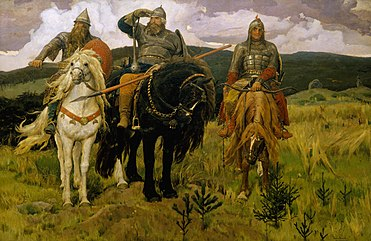
\includegraphics[width=0.49\textwidth]{img/tri_bogatyrya.jpg}
    \end{center}
    \caption{Картина «Три Богатыря» ВМ Васнец\'{о}ва (слева направо: Добрыня Никитич, Илья Муромец и Алёша Попович), ВикипедиЯ.}
\end{wrapfigure}
В центре картины изображён Илья Муромец, народный любимец, герой русских был\'{и}н. Не всем известно, что Илья Муромец не сказочный персонаж, а реальное историческое лицо. История его жизни и \explainDetail{р\'{а}тных}{р\'{а}тный}{military} \explainDetail{п\'{о}двигов}{п\'{о}двиг}{exploit, feat} -- это реальные события. \explain{Впосл\'{е}дствии}{subsequently}, закончив свои труды по охране родины, он стал монахом Киево-Печёрского монастыр\'{я}. Был причислен к л\'{и}ку свят\'{ы}х\footnote{was canonised}. Васнецов эти факты знал, создав\'{а}я образ Ильи Муромца. «\explainDetail{Матёр}{матёрый}{mature, fully grown, hardened} человек Илья Муромец» -- говорит былина. А на картине Васнецова мы видим могучего воина и при том \explainDetail{бесх\'{и}тростного}{бесх\'{и}тростный}{ingenuous, silly} открытого человека. В нём \explainDetail{сочетаются}{сочетаться}{combine} исполинская сила и \explain{великод\'{у}шие}{generosity, magnanimity, goodness}. «А конь под Ильёй \explain{лютый}{fierce} зверь» -- продолжает сказание. \explainDetail{Мощная}{мощный/-ая/-ое}{powerful} фигура коня, изображённого на картине с массивной металлической цепью вместо упряжки, \explainDetail{свид\'{е}тельствует}{свид\'{е}тельствовать}{testify; свидетель: witness} об этом.

Добрыня Никитич по народным преданиям был очень образ\'{о}ванным и \explainDetail{м\'{у}жественным}{м\'{у}жественный}{manly} человеком. С его личностью связано много чудес, наприм\'{е}р, заговорённая броня\footnote{charmed armor} на его плечах, \explain{волш\'{е}бный}{magic} меч-кладенец. Добрыня изображён таким как и в былинах -- величавым, с тонкими, благородными чертами лица, подчёркивающими его культурность, образ\'{о}ванность, \explain{решительно}{decisively} вынимающий меч из \explain{н\'{о}жен}{sheath} с готовностью \explainDetail{бр\'{о}ситься}{брос\'{а}ться/бр\'{о}ситься}{rush} в бой, защищая свою родину.

Алёша Попович \explain{по сравнению с}{as compared with} товарищами молод и строен. Он изображён с \explainDetail{л\'{у}ком}{лук}{bow} и стрелами в руках, но \explain{прикреплённые}{attached} к \explainDetail{седлу}{седло}{saddle} гусли свидетельствуют о том, что он не только бесстрашный воин, но и \explain{гусляр}{player of the musical instrument ``gusli''}, песенник, весельчак. В картине много таких деталей, которые характеризуют образы её персонажей.

Упряжки коней, одежда, амуниция не \explainDetail{вымышленные}{в\'{ы}мышленный/-ая/-ое}{imaginary, fictitious}. Такие образц\'{ы} художник видел в музеях и читал их описания в исторической литературе. Художник \explain{мастерски}{masterfully} передаёт состояние природы, как бы предвещающей о наступлении опасности. Но богатыри представляют собой \explainDetail{надёжную}{надёжный/-ая/-ое}{reliable} и мощную силу защитников родной земли.




\subsection{Картина «Алёнушка» ВМ Васнец\'{о}ва}
% https://muzei-mira.com/kartini_russkih_hudojnikov/1321-opisanie-kartiny-bogatyri-tri-bogatyrya-vasnecova-1898.html

Алёнушка, печальная девочка у \explainDetail{пруда}{пруд}{pond} --- одна из любимых всеми картин В. Васнецова. Художник уд\'{а}чно использует сказочный сюжет, чтобы \explainDetail{раскрыть}{раскрывать/раскрыть}{to open/to discover} сложный и неоднозначный русский характер.

\begin{wrapfigure}{l}{0.4\textwidth}
    \begin{center}
        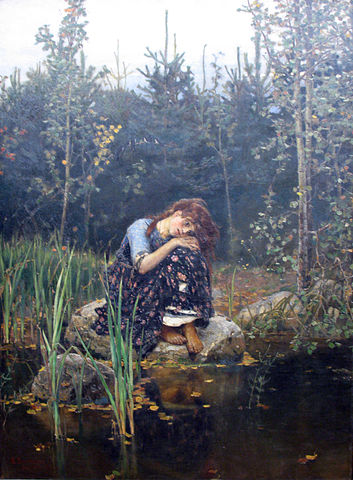
\includegraphics[width=0.38\textwidth]{img/alyonushka.jpg}
    \end{center}
    \caption{Алёнушка, ВикипедиЯ}
\end{wrapfigure}
Грусть девочки очень взрослая. Печаль в её глазах граничит с \explainDetail{отчаянием}{отч\'{а}яние}{despair}. Неубранные рыжие волосы, тёмные глаза, нежно-алые губы --- формируют легко читаемый образ ребёнка с тр\'{у}дной судьб\'{о}й.
В Алёнушке совсем нет ничего \explainDetail{сказочного}{сказочный}{fabulous, fairytale-like}, фантастического.
С\'{о}бственно, вся ск\'{а}зочность сюжета подчеркнута лишь одной деталью --- группой \explainDetail{ласточек}{л\'{а}сточка}{swallow}, сидящих над головой \explainDetail{героини}{героиня}{heroine}. Этим с\'{и}мволом (как известно, л\'{а}сточки символиз\'{и}руют над\'{е}жду) художник \explainDetail{уравновешивает}{уравновешивать/уравновесить}{to balance --- уравнов\'{е}шиваю/-ешь/-ют; уравнов\'{е}шу/-ишь/-ят} полный \explainDetail{тоск\'{и}}{тоск\'{а}}{yearning, longing} \'{о}браз героини, даёт надежду на счастливый финал старой русской сказки.

Васнецов нап\'{о}лнил \explain{ф\'{о}новый}{background} пейзаж атмосферой тишины и гр\'{у}сти.
Отлично удал\'{и}сь художнику в\'{о}дная \explain{гладь}{smooth surface} пруда, \explainDetail{камыш\'{и}}{камыш}{reed}, осока, \explainDetail{ели}{ель}{fir tree}.
Всё \explainDetail{неподв\'{и}жно}{неподв\'{и}жный/-ая/-ое}{still, motionless}, тихо, спокойно.
Даже пруд отраж\'{а}ет героиню очень деликатно, \explain{слегк\'{а}}{slightly}.
Чуть трепещут молодые \explainDetail{ос\'{и}ны}{ос\'{и}на}{aspen}. \explainDetail{Едва}{едв\'{а}}{barely, hardly} \explain{хмурится}{turns gloomly} ос\'{е}ннее небо.
Тёмные, зелёные тона пейзажа контрастируют с \explainDetail{румянцем}{румянец}{blush} на лице героини, а ос\'{е}нняя грусть --- с яркими цветами на юбке Алёнушки. Зритель чувствует: ещё мгнов\'{е}ние и сказка прод\'{о}лжится\dots







\subsection{Картина «Витязь на распутье»}

Виктор Михайлович Васнецов с циклом работ, \explain{посвященных}{dedicated (посвященный + \textit{дат.})} сюжетам русских сказок и былин, оказался \explainDetail{новатором}{новатор}{innovator} в этой области \explainDetail{изобразительного искусства}{изобраз\'{и}тельное искусство}{visual art}. За ним закрепилась репутация «художника-сказочника», он настолько проникся духом русской старины и былинного времени, что свой московский дом построил в виде деревянной избы (сейчас там находится мемориальный музей \explainDetail{живоп\'{и}сца}{живоп\'{и}сец}{painter, artist}).


Картина «В\'{и}тязь на расп\'{у}тье» \explain{отч\'{а}сти}{partly} является и отражением судьбы Васнецова.
Будучи \explainDetail{пр\'{и}знанным}{пр\'{и}знанный}{recognised} художником-передвижником, он, как и его товарищи, \explainDetail{исполнял}{исполнять/исполнить}{performed} жанровые композиции в духе остросоциальных тем, волновавших общество в 1870-1890-х.
Но завладевшая им сказочная тематика диктовала \explainDetail{ин\'{о}е}{ин\'{о}й/ин\'{а}я/ин\'{о}е}{(определительное местоимение) другой, отличный от данного; (неопределённое местоимение) некоторый. See \href{https://ru.wiktionary.org/wiki/\%D0\%B8\%D0\%BD\%D0\%BE\%D0\%B9}{wikictionary.org:иной}.} развитие творчества. Живописец уход\'{и}л от проблем современности и \explain{погружался}{plunge, dive} в мир русской старины, рискуя быть \explainDetail{осужденным}{осужденный}{convicted}.

\begin{wrapfigure}{l}{0.58\textwidth}
    \begin{center}
        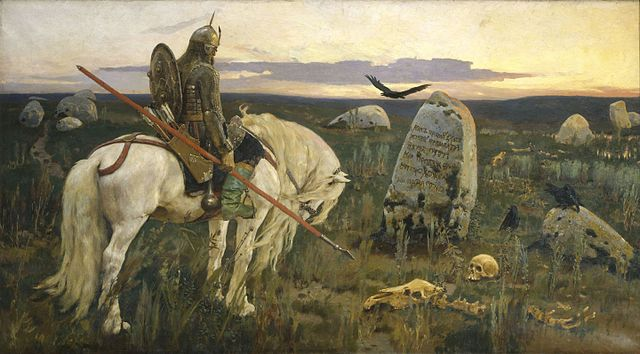
\includegraphics[width=0.57\textwidth]{img/TheKnightAtTheCrossroads.jpg}
    \end{center}
    \caption{Витязь на распутье, ВикипедиЯ}
\end{wrapfigure}
Выбор пути как один из \explain{роков\'{ы}х}{fatal} вопросов человеческой жизни на крупноформатном \explainDetail{холсте}{холст}{canvas} мастера приобрел эпическое звучание.
Перед камнем-предсказателем согнулся под тяжестью фатального \explainDetail{пророчества}{пророчество}{prophecy} опечаленный витязь. \explainDetail{Зловещий}{зловещий}{sinister} в\'{о}рон, садящееся красное солнце нагнетают\footnote{build up the atmosphere} атмосферу. \explainDetail{Нам\'{е}ренный}{нам\'{е}ренный}{intentional} отказ от \explainDetail{изображения}{изображение}{depiction} дороги (как выхода из трудности) художником сделан для того, чтобы показать \explain{неотврат\'{и}мость}{inevitability} судьбы.

